\documentclass{article}%
\usepackage[T1]{fontenc}%
\usepackage[utf8]{inputenc}%
\usepackage{lmodern}%
\usepackage{textcomp}%
\usepackage{lastpage}%
\usepackage[head=40pt,margin=0.5in,bottom=0.6in]{geometry}%
\usepackage{graphicx}%
%
\title{\textbf{Maestros en Cojedes marcharon para rechazar tabulador salarial}}%
\author{El Nacional Web}%
\date{16/10/2018}%
%
\begin{document}%
\normalsize%
\maketitle%
\textbf{URL: }%
http://www.el{-}nacional.com/noticias/protestas/maestros{-}cojedes{-}marcharon{-}para{-}rechazar{-}tabulador{-}salarial\_255940\newline%
%
\textbf{Periodico: }%
EN, %
ID: %
255940, %
Seccion: %
Protestas\newline%
%
\textbf{Palabras Claves: }%
Cojedes, Economía, Protestas, Gobierno\newline%
%
\textbf{Derecho: }%
2.3%
, Otros Derechos: %
NO\_TIENE%
, Sub Derechos: %
2.3.4%
\newline%
%
\textbf{EP: }%
SI\newline%
\newline%
%
\textbf{\textit{Los docentes aseguran que el sueldo no les alcanza para cubrir sus gastos}}%
\newline%
\newline%
%
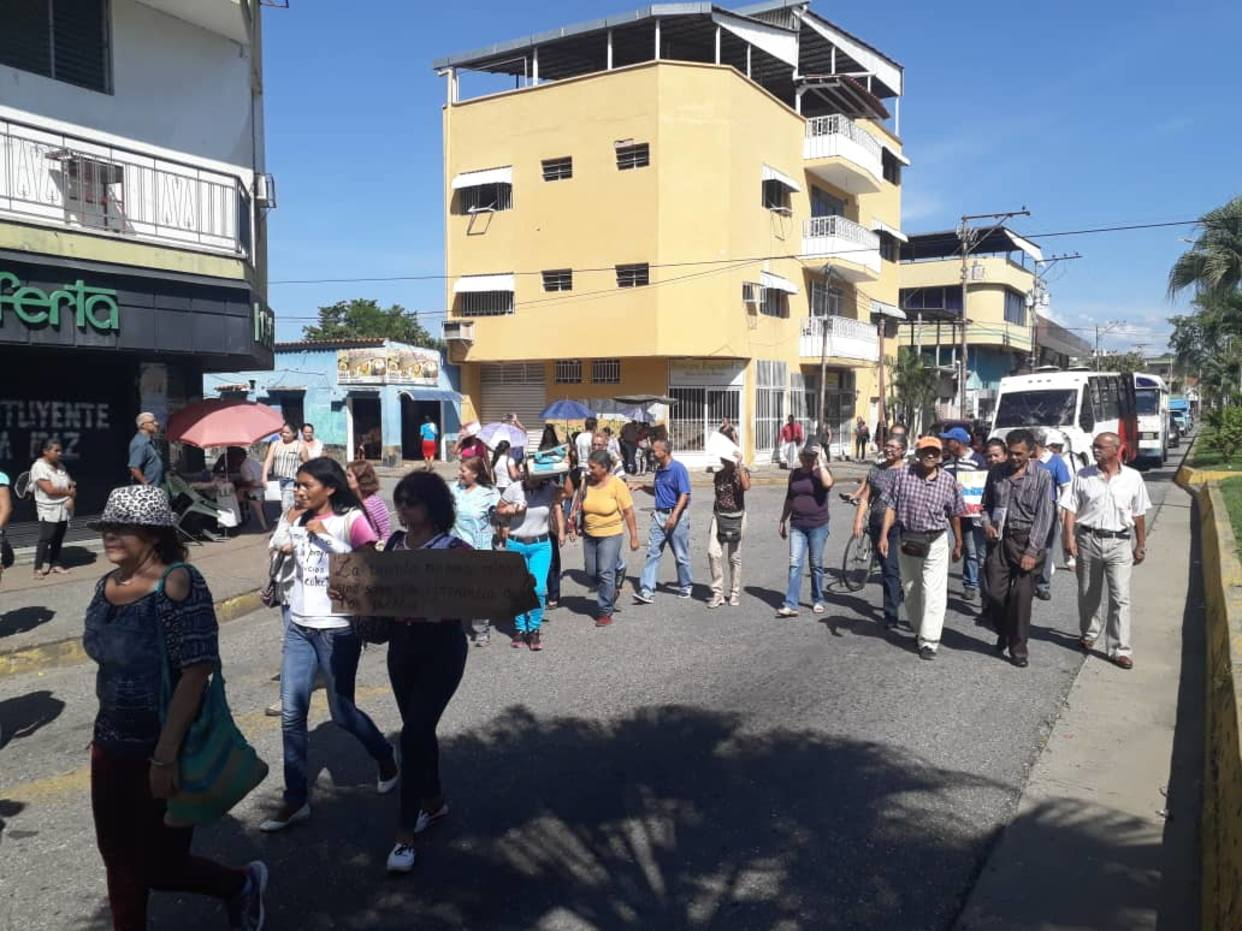
\includegraphics[width=300px]{80.jpg}%
\newline%
%
Maestros de San Carlos, estado Cojedes, marcharon este martes por las principales calles de la entidad como forma de protesta contra el tabulador salarial impuesto por el gobierno nacional.%
\newline%
%
Reportes de Twitter indican que los docentes se trasladaron a la Defensoría del Pueblo para entregar un documento. Aseguran que el suelo no les alcanza para cubrir sus necesidades.%
\newline%
%
Los manifestantes portan pancartas y gritan consignas para exigir un aumento de salario.%
\newline%
%
\end{document}